\cleardoublepage

\newrefsection

\chapter{外文翻译}

本章节节选了《SpecDoctor: Differential Fuzz Testing to Find Transient Execution Vulnerabilities》的摘要、介绍、背景、问题与挑战、系统设计等五个部分进行翻译, 该文章被计算机安全领域顶会 ACM SIGSAC Conference on Computer and Communications Security,2022 所收录。我们选择这篇文章作为现有的处理器瞬态执行漏洞测试程序生成框架的案例。

\section*{摘要}

瞬态执行漏洞因其能破坏 CPU 的基本安全假设而对软件系统安全产生了重要影响。为了能在芯片制作阶段之前尽早发现和修复这些漏洞,RTL 开发阶段的瞬态执行漏洞检测就显得尤为重要。\par

本文提出了一种用于处理器瞬态指令漏洞检测的 RTL 自动模糊测试工具 SpecDoctor。具体来说,SpecDoctor 设计了一种可以测试所有不同场景的瞬态执行漏洞(例如,Meltdown、Spectre、Foreshadow)的模糊测试模板。然后,SpecDoctor根据RTL上下文中的各个漏洞约束依次执行多阶段模糊测试,从而进行高效的漏洞查找。\par

我们在两个乱序 RISCV 处理器 Boom 和 NutShell-Argo 上进行 SpecDoctor 的实现和评估。在评估的过程中,SpecDoctor 除了发现了与之前的工作有类似攻击方式的瞬态执行漏洞之外,还发现了两个使用其他攻击方式的有趣变体:Boombard 和 Birgus。Boombard 利用 RISC-V Boom 中的一个未知的实现错误触发瞬态执行漏洞;Birgus 在 NutShell CPU 上使用一个独特的指令组合构造了通过端口竞争侧信道泄露数据的 Spectre 攻击。我们向开发者汇报了这两个漏洞,并得到了开发人员的认可,这正好说明了 SpecDoctor 具有强大的现实影响力。

\section*{CCS 分类}
· 安全和隐私 $\longrightarrow$ 测信道分析和时间测量

\section*{关键词}
瞬态执行漏洞;模糊测试;差分测试

\section{介绍}

瞬态执行漏洞是现代处理器中的关键漏洞。自从 Meltdown 和 Spectre 被首次披露以来,其他许多的瞬态执行漏洞,如 ForeShadow、RIDL、FPVI、CacheOut等也被陆续发现。虽然这些漏洞严重损害了受影响的CPU上软件的安全性,但因为这些补丁植根于CPU的微架构,导致开发商无法快速的发布漏洞补丁。\par

投机执行最初被用于最大化CPU性能,瞬态执行漏洞的产生与之高度相关。具体来说,CPU尝试预测早期指令的运行结果,然后在假设预测结果正确的情况下执行后续指令。但是,如果预测错误,CPU会回滚后续执行的指令,以保持执行的正确性。这些被回滚的指令被称为瞬态指令。这个回滚在架构层面是不可见的,所以瞬态执行不会损害CPU的执行正确性——它只改变了处理器的微架构状态。但问题在于,人们已经发现了各种用于跟踪瞬态执行指令引发的微架构状态变化的技术。由于这些瞬态指令是人为引入的错误预测导致的,它们本不应该被执行,因此瞬态指令的执行结果可能包含安全敏感数据,这违反了CPU的基本安全隔离保证。\par

虽然已经有了几种可以在现成的cpu(即已经生产的cpu)上自动检测这些漏洞的方法,但在RTL开发阶段进行的检测方法并没有得到太多关注。RTL开发阶段的漏洞检测为处理器提供了一个在CPU芯片制造和发布之前进行漏洞修复的机会,这使得该工作尤为重要。因为这些漏洞是根植于硬件芯片的,所以一旦芯片被制作完成,这些漏洞的修复将变得异常困难。由于硬件的不可修复性,许多处理器(如 x86)上的瞬态执行漏洞仍然没有被修复(或部分修复)。\par

鉴于前期检测的重要性,本文重点研究了如何采用流行的模糊测试来实现基于rtl的瞬态执行漏洞检测。与传统的模糊技术相比,我们发现使用模糊测试进行瞬态执行漏洞自动识别有两个独特的挑战。首先,瞬态执行漏洞可以在各种威胁模型和上下文设置中被启动。具体来说,因为这些漏洞利用了底层的硬件,运行在CPU上的所有软件实体(即用户程序、内核或飞地)都可能是受害者或攻击者。\par

此外,根据瞬时执行的执行方的不同,攻击可以有不同的构造方式——例如,Meltdown 中的瞬态执行是在攻击者一方执行的,而 SpecDocotr 中的瞬态执行是在受害者一方执行的。此外,各种CPU设置,如页表表项设置(例如,ForeShadow)等也会影响瞬态攻击的执行。这些问题在传统的模糊测试领域是不常见的,因为传统模糊主要关注如何扩展输入测试的覆盖率,它们的威胁模型和设置在目标确定后是固定的(例如,AFL 和  Syzkaller 在突变文件输入或系统输入时,其运行环境是不变的)。\par

第二个挑战是,瞬态执行漏洞是难以被检测到的。众所周知,为了触发这些漏洞,需要触发两个非法行为: 1)触发瞬态执行,2)构建微体系结构侧信道。然而,我们不清楚如何显式地将这些非法行为表示为RTL文件中的可编程约束。更重要的是,为了完成瞬态执行攻击,这两个违法行为需要被串联执行,这使得瞬态执行漏洞的检测更加困难。\par

在本文中,我们提出了一种能自动发现CPU RTL中瞬态执行漏洞的工具。SpecDoctor 是一个成熟的RTL模糊测试工具,它能找到在所有可能的上下文设置中都能执行的瞬态执行攻击。SpecDoctor 通过以下两种方法解决上述挑战。首先,SpecDoctor对所有的威胁模型和硬件设置实现了一个通用模板。SpecDoctor为了能在给定模板上涵盖所有瞬态执行漏洞,提供了全面的配置选项。其次,SpecDoctor基于配置的模板设计了一个多阶段的模糊框架,来依次解决瞬态执行漏洞中的每个违例约束。为了检测RTL层级中的非法行为,SpecDoctor监视单个RTL结构来检测所有瞬态执行的发生。然后,它实现了一个差异测试框架来识别微架构时间侧信道,同时选择性地对RTL组件进行监控。基于以上步骤,SpecDoctor最后输出一个针对给定 CPU 的完整瞬态执行攻击PoC。使用这种攻击poc,我们能够一模一样的重现这个漏洞。\par

我们在两个真实的开源RISC-V 乱序流水线处理器 Boom和NutShell-Argo上分别实现和评估了SpecDoctor。最后,SpecDoctor在这些cpu上发现了与之前工作所发现的攻击有相似攻击向量的瞬态执行漏洞。除此之外,SpecDoctor 发现了两种利用之前工作未曾发现的攻击方式进行瞬态执行攻击的攻击变体:i)RISC-V Boom上的BoomBoard,和ii)NutShell上的Birgus。所有这些漏洞都获得了相应开发人员的认可,其中 BoomBoard 获得了一个CVE号。\par

BoomBoard在RISC-V Boom处理器中发现的的Meltdown变体。BoomBoard最值得注意的方面在于,它利用了RISC-V Boom中的一个实现错误——即,存在不遵循处理器实现规范的RTL实现行为。根据RISC-V Boom规范,Boom CPU的分支预测器内部不应该存在侧信道。但是,SpecDoctor在RISCV BOOM的分支预测器逻辑电路中发现了一个没有遵循处理器实现规范的实现错误,并通过利用该实现错误触发了一个严重的瞬态执行漏洞。BoomBoard攻击向硬件工程师提出了如下警告:如果想要构建一个真正安全的 CPU,硬件工程师们不应该仅仅止步于对静态的CPU规范手册的遵守,更应该对他们实现的 RTL 进行动态的测试验证。\par

Birgus是在RISC-V NutShell中发现的一个Spectre变体,它通过使用一个之前从未被注意的小型部件,构建了一个端口争用侧信道。我们发现,端口竞争侧信道相关的指令组合在之前的工作中已经被广泛研究了。为了缓解端口竞争侧信道问题,一些与之相关的指令组合已经被列入了黑名单。但在这一方面,Birgus提供了一个在之前的工作中没有发现的新的指令组合,这意味着当前的CPU仍然很容易遭受到端口竞争侧信道的攻击。因此,Birgus说明了,即使处理器经过了基于模式的硬件验证(例如,回归测试),并采用了一些能缓解Spectre攻击的策略,它们内部仍然可能存在安全隐患。尽管SpecDoctor没有总结出需要被检查的小型部件的集合,Birgus还是建议我们,如果想要阻止瞬态执行漏洞的产生,我们还有大量的验证工作需要持续不断地进行下去。\par

\section{背景}

本节提供了理解SpecDoctor所必需的瞬态执行攻击(2.1)和CPU微架构(2.2)的背景知识。然后,我们简要描述了模糊测试技术(2.3)的基础知识。

\subsection{瞬态执行攻击}

瞬态执行是指瞬态指令的执行,这些指令会改变处理器微架构的状态,但不会改变架构状态。因此,从架构的角度来看,瞬态指令并没有被执行,故而瞬态指令不会影响CPU执行的正确性。但是,如果攻击者能够通过瞬态指令学习到微体系结构状态,就可以造成严重的安全隐患,这一行为被称之为瞬态执行攻击。具体来说,瞬态执行攻击允许攻击者通过精心操纵数据流和控制流触发瞬态执行(例如,错误的投机执行或错误的分支预测),然后通过读取微架构状态中残留的秘密数据相关的痕迹,来还原秘密数据。由于乱序执行和各种投机执行等优化技术的广泛使用,几乎所有的现代cpu在瞬态执行攻击前面都是脆弱的。\par

\textbf{已知的瞬态执行攻击。}本文通过以下几个层面对瞬态执行攻击进行介绍: 1)触发瞬态执行,2)访问秘密数据,3)通过微体系结构的侧信道泄露数据。\par

可以使用Spectre或Meltdown类型的攻击出发瞬态执行。具体来说,Spectre类型通过操纵控制流和数据流的预测来触发瞬态执行。例如,Spectre毒害CPU的分支预测器来触发瞬态执行,而Ret2spec则通过毒害返回地址堆栈。另一方面,Meltdown类型利用延迟的权限检查,如检查页表条目中的标志位,或检查浮点寄存器的权限。\par

为了访问秘密数据,攻击者必须绕过由软件(例如边界检查)或硬件(例如页面权限检查)强制执行的安全边界检查。Spectre 攻击通过触发瞬态执行来操作控制流,从而绕过软件强制执行的安全检查。而 Meltdown 类型则绕过由硬件原语强制执行的安全检查。微体系结构数据采样(即MDS)攻击在瞬态执行窗口访问了 CPU 共享缓冲区中的秘密数据,它也可以被分类为 Meltdown 类型。\par

最后,攻击者通过滥用微体系结构侧信道泄露秘密数据。已知cpu有各种侧信道,包括缓存、分支预测器,甚至执行端口。很多攻击基于易受攻击的CPU组件在不同环境下泄露秘密数据(例如,针对 Dcache 侧信道的刷新和重加载、启动模式和探测模式等)。由于CPU组件的复杂性和共享特性,更多的侧信道正在被不断发掘出来。\par

\subsection{CPU 微架构}

CPU微体系结构是一种遵循预定义的指令集架构(ISA)的处理器RTL实现。由于CPU需要支持算术运算等简单运算到虚拟地址转换的复杂运算的整个指令集架构,因此它包含了大量的组件和逻辑电路。\par

\begin{figure}[!h]
    \centering
    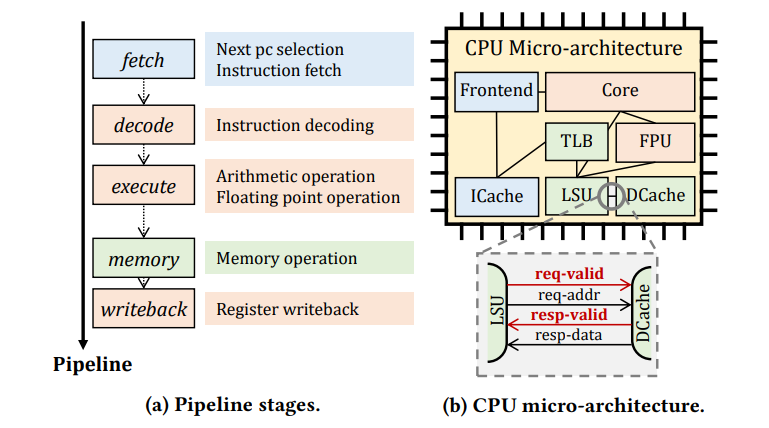
\includegraphics[width=\linewidth]{figure/proposal/specdoctor-figure1.png}
    \caption*{图1:流水线阶段设计及其在CPU中的RTL实现。为执行一条指令,CPU中的模块通过连续地交换信号相互配合。}
\end{figure}

\textbf{CPU流水线实现。}CPU为指令执行提供了多阶段(例如,获取、解码、执行等)的流水线,而这些流水线阶段的设计最终会被具体化为CPU中的RTL实现。例如,如图1所示,图1-(b)中的前端负责下一个pc的选择和指令获取(即在图1-(a)中的获取),Core 负责算术操作(即在图1-(a)中执行),负载存储单元(即LSU)和DCache负责响应内存请求(即图1-(a)中的内存)。因此,指令在各阶段中依次执行,由各个模块完成其对应阶段被配分配的工作(例如,获取指令)。\par

同时,CPU中的模块通过电线相互连接进行信号交换,相互协同来完成指令需要的服务。特别注意,模块通过交换控制信号来表示请求或响应。例如,在图1-(b)中,LSU通过使能req-valid信号向DCache发起内存请求,通过req-addr发送请求的地址信号。然后,当resp-data数据信号上的数据准备就绪时,DCache 使能resp-valid信号来响应请求。根据数据存放的的位置不同(例如,在L1、L2缓存或内存),valid信号的响应也会相应的被延迟或提前。因此,控制信号的交互信息可以反映一个任务阶段的执行结束。\par

\textbf{乱序执行和重排序缓冲区。}现代cpu采用乱序执行的方式提高处理器性能。虽然从架构层的角度来看,指令应该按顺序被执行,但是CPU允许指令在CPU内部执行的时候是乱序的。在乱序CPU中,所依赖的操作数已经准备就绪的指令可以被立刻发射,以便CPU可以提早执行这些指令。同时,CPU会将获取的指令按顺序排列在重排序缓冲区(RoB)中,以此保持指令在架构层中的执行顺序。RoB通过保存指令并按顺序提交它们的方式来保持程序员可见的架构顺序。\par

但是,不是所有RoB中的指令都是会被提交的,比如那些在ISA语境中不应该被执行的指令(即瞬态指令)。当这些瞬态指令(例如,分支错误预测)出现时,RoB将刷新触发指令(例如,分支指令)之后的指令队列条目,并将队列尾部回滚到正确指令的位置。因此,虽然瞬态指令会被CPU中各部分触发,但是只需要RoB一个部件就可以实现指令执行顺序同步的功能。\par

\subsection{模糊测试}

模糊测试可以说是最有效的软件错误检测技术。模糊测试背后的关键思想是不断地用简单随机生成的输入测试目标程序。在迭代循环时,模糊器通过保存触发有趣行为(例如,扩展代码覆盖)的输入,并对它们进行突变的方式以进一步找到角情况。从AFL开始,模糊测试工具就从各种程序(比如内核、管理程序,甚至是CPU)中发现了大量错误。\par

\textbf{差分模糊测试。}模糊测试工具需要一种检测机制来检测错误或者说检测异常行为。虽然内存损坏等异常行为很容易被内存错误检测器(如ASAN)捕获,但那些没有表现出明显异常行为的语义错误则很难被检测到。因此,差分测试被先前关于识别语义bug的工作所采用,它通过比较具有相同功能和执行目标的多个程序的执行结果(例如,文件系统,JVM)进行错误检测。由于这些程序应该为相同的输入返回相同的结果,所以如果它们显示不同的输入-输出关系,我们可以认定这是一个bug。差异测试已经被合并到模糊测试当中(即图2),差异模糊测试技术也已被广泛用于查找文件系统等程序中的bug。\par

\begin{figure}[!h]
    \centering
    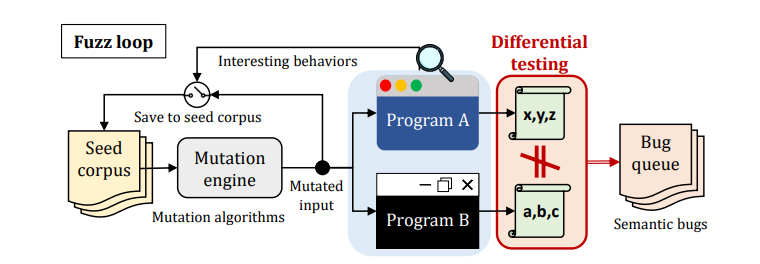
\includegraphics[width=\linewidth]{figure/proposal/specdoctor-figure2.png}
    \caption*{图2:差分模糊测试的基本工作流程。}
\end{figure}

\section{SpecDoctor的挑战}

基于瞬态执行漏洞独有的特性,发现瞬态执行漏洞需要面临两个挑战。第一个挑战是,这些漏洞具有不同的威胁模型和设置(C1)。第二,这些漏洞难以在RTL上下文(C2)中定义漏洞约束。我们将在下文中依次详细阐述这两个挑战。\par

\textbf{C1.各种威胁模型和设置。}自Spectre和Meltdown被发现以来,越来越多的瞬态执行漏洞在各种不同的威胁模型(即受害者和攻击者的特权)和上下文设置(即内存设置或禁用/启用SMT)下被发现。这表明,为了检测所有瞬态执行漏洞,SpecDoctor 需要能概括所有可能的配置,包括威胁模型、内存设置和瞬态执行的上下文。\par

现在我们以类似Spectre的漏洞和类似Meltdown的漏洞为例来突出这一挑战的难度。在漏洞类似Spectre的情况下,SpecDoctor应做如下配置: (i)威胁模型:内核是受害者,用户是攻击者;(ii)内存设置:配置页面表,禁止用户访问内核内存;(iii)上下文:从受害者的上下文启动瞬态执行。相反,在漏洞类似Meltdown的情况下,SpecDoctor应做如下配置: (i)威胁模型:与Meltdown漏洞相同;(ii)内存设置:内核的内存应该受到保护,但它应该被映射到用户地址空间;(iii)上下文:应该从攻击者的上下文启动瞬态执行。\par

此外,因为底层硬件有大量的可用配置(例如,飞地、SMT或页表项设置),这一挑战变得更加严峻。例如,ForeShadow 发现,可以通过和 Meltdown 类似的机制对飞地进行攻击。Medusa 利用不同CPU的内存缓冲区引入 ZombieLoad 的变体。\par

\textbf{C2.检测RTL中的漏洞约束。}因为内存损坏bug有一个相当简单的漏洞约束(即,一个内存指令应该访问一个有效的内存区域),所以传统的模糊测试技术可以利用这个简单的约束来进行检测bug。\par

然而,瞬态执行漏洞是语义级别的漏洞,它们在RTL层中没有检测违例的确切约束。更糟糕的是,这些漏洞可以通过具有不同根本原因的不同指令来启动,这使得它们很难被表述为一个简单且易于检测的约束。具体来说,之前的工作粗略地描述了如下的瞬态执行漏洞约束: (i)攻击指令被瞬态执行;(ii)攻击指令构建微体系结构时间侧信道,以此泄露秘密数据。虽然这些约束说明了瞬态执行漏洞的高级特征,但目前尚不清楚如何在RTL上下文中编程这些约束。\par

以约束(i)为例,瞬态执行可以由各种RTL组件触发,例如,分支预测错误、内存访问缺页异常、访存指令地址不对齐等。由于它们分别是由不同的RTL组件导致的,因此尚不清楚如何对它们进行全面的检测约束(i)。此外,因为CPU包含了很多不同的时间侧信道,例如数据和指令缓存、TLB、分支预测器等,因此这些约束总能被某些 RTL 组件满足。但正如前文所提到的,想要检测所有不同RTL组件有无违反约束,这对于 SpecDoctor 是很困难的。\par

\textbf{SpecDoctor的解决方法。}为了解决上述挑战,我们基于以下两种方法设计了SpecDoctor。为了解决第一个挑战(即,C1),SpecDoctor提供了一个能配置所有硬件设置(例如,虚拟内存)的通用模板,它通过选择一组配置(即,威胁模型和瞬态执行的上下文)来配置攻击方式。SpecDoctor全面定义了配置选项,以便可以覆盖所有的瞬态执行漏洞(更多细节见4.1)。\par

为了处理第二个问题(即C2),针对约束(i),SpecDoctorcor首先通过检测关键的RTL组件来检测瞬态执行的发生。这使得SpecDoctor可以仅通过监控单个RTL组件,就捕获到所有瞬态执行指令。为了可以检测约束(ii),SpecDoctor选择性地监测能构建时间测信道的RTL组件,并结合差分测试的方法进行检测。更重要的是,SpecDoctor执行多阶段模糊测试(更多细节见4.2、4.3和4.4),其中每个阶段检测对应的违例约束,然后将所有阶段的结果按顺序链接在一起,从而允许SpecDoctor有效地找到瞬态执行漏洞。\par

\section{SpecDoctor 的设计}
SpecDoctor是一种用于瞬态执行漏洞查找的全自动处理器 RTL 模糊测试工具。对于给定的处理器RTL,SpecDoctor能自动地对所有可能的威胁模型配置进行模糊测试,并找到发动瞬态执行攻击的具体PoC,进而准确地确认和复现漏洞。\par

\textbf{概述。}为了系统地发现瞬态执行漏洞,我们设计的 SpecDoctor 工具由四个阶段构成,如图3所示。在阶段1中,SpecDoctor通过选择诸如威胁模型和瞬态执行的上下文等配置选项确定瞬态攻击的类型。SpecDoctor 会根据攻击的威胁模型和上下文,按照对应的基础模板设置虚拟地址和硬件原语,以保护机密数据。\par

\begin{figure}[!h]
    \centering
    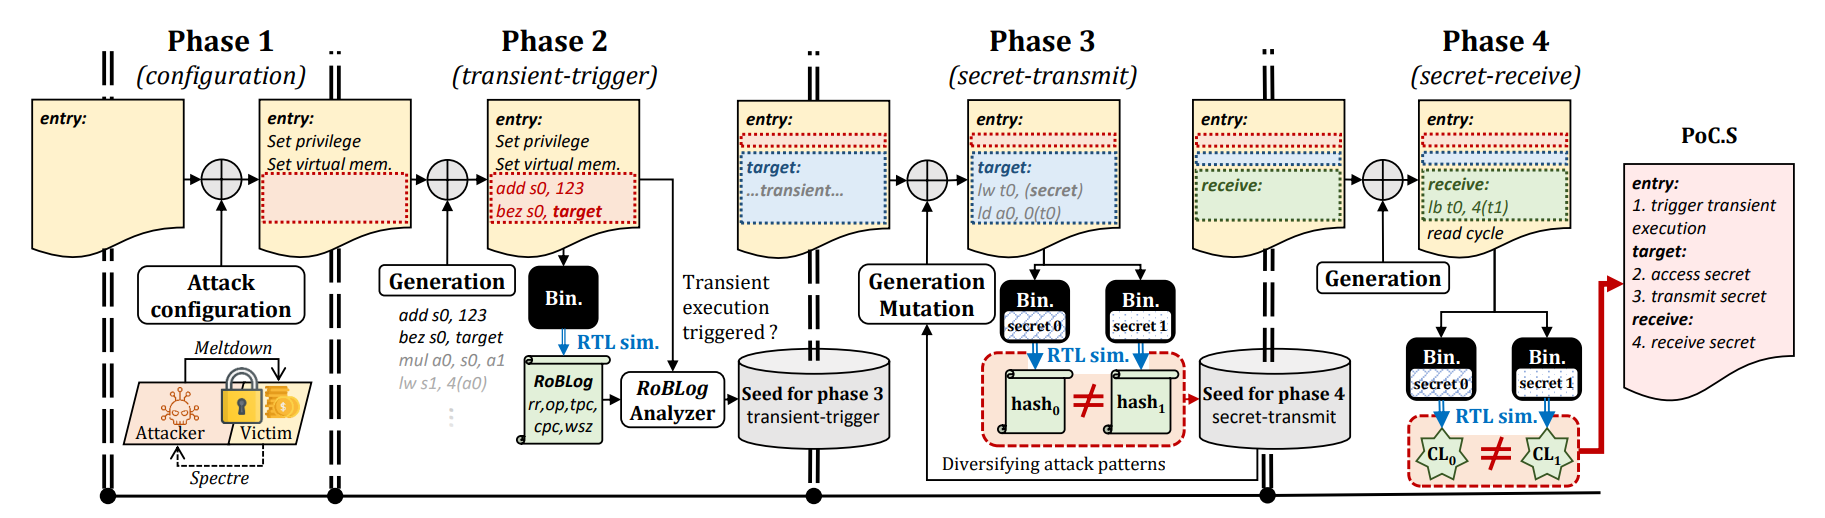
\includegraphics[width=\linewidth]{figure/proposal/specdoctor-figure3.png}
    \caption*{图3:SpecDoctor瞬态执行漏洞差分测试框架。}
\end{figure}

根据给定的模板,SpecDoctor依次生成满足关键漏洞约束的指令序列,并最终得到可以触发瞬态执行攻击的具体 poc。在阶段 2 中,SpecDoctor 找到可以触发瞬态执行窗口的指令序列。阶段3根据阶段2得到的测试用例,随机生成瞬态指令,试图找到能瞬态访问和传输秘密数据的指令组合。在阶段 4 中,SpecDoctor 通过随机生成指令的方式,寻找可以还原阶段3泄露的秘密的指令序列,最终实现完整的瞬态执行攻击。\par

\subsection{阶段1:攻击配置}

由于瞬态执行攻击可以在各种环境中执行,因此SpecDoctor需要为攻击者和受害者设置各类不同的攻击上下文和特权来测试所有可能的攻击场景。图4-(a)总结了在这个阶段可能的威胁模型配置选项,其关键设计在于使SpecDoctor能够测试所有可能的攻击场景,同时避免不必要的复杂场景。\par

\begin{figure}[!h]
    \centering
    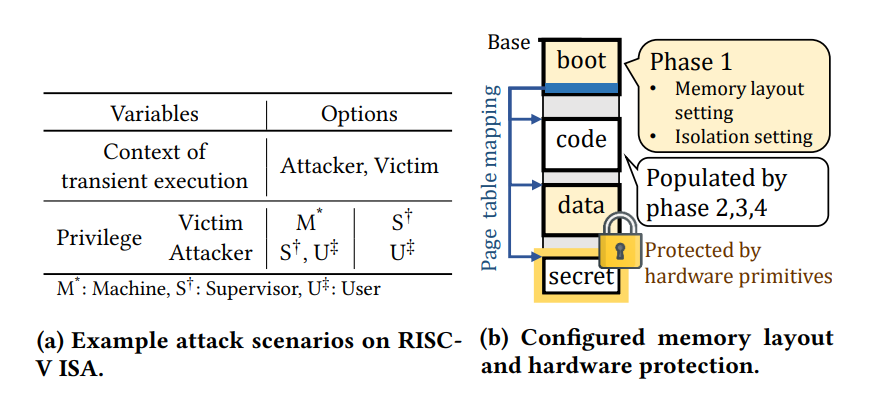
\includegraphics[width=\linewidth]{figure/proposal/specdoctor-figure4.png}
    \caption*{图4:SpecDoctor 阶段 1 的配置。}
\end{figure}

\textbf{瞬态执行的上下文。}瞬态执行攻击可在两种不同的上下文中执行——攻击者的上下文或者受害者的上下文。由于不同的上下文会影响攻击的启动方式(因为SpecDoctor必须根据上下文设置正确的执行权限),因此SpecDoctor提供了用于指定瞬态执行上下文的配置选项。在执行攻击者的代码时触发崩溃或MDS的瞬态攻击等场景属于在攻击者的上下文发动攻击,在执行受害者的代码时触发瞬态执行等场景属于在受害者的上下文发动攻击。\par

\textbf{攻击者和受害者的权限。}为了对攻击者和受害者的特权进行指定设置,SpecDoctor提供了对应的配置选项。RISCV提供了三种可用的特权级:机器模式M、监督者模式S、用户模式U,分别对应于飞地、内核和用户进程。因为攻击者的目标往往是获得特权设计不允许访问的更高特权区域的机密数据,所以这里我们假设受害者总是拥有比攻击者更高的特权。针对受害者特权级的不同,我们使用不同的硬件原语对机密数据进行保护。\par

\textbf{初始化内存区域。}因为测试程序是运行在一个基本裸露的CPU上的,所以SpecDoctor需要先对内存区域进行初始化。SpecDoctor分配了四个物理内存区域,如图4-(b)所示,分别是引导段、代码段、数据段、秘密数据段。在引导段中,SpecDoctor会放置初始配置代码,例如用于启用和初始化虚拟内存布局的代码,以及设置异常处理程序入口的代码等等。在初始化虚拟内存时,SpecDoctor会配置页表,让监控程序和用户程序能够在各自的地址空间中运行。SpecDoctor随机分配页表权限标志(即读、写、执行和用户标志),以便测试所有可能的页表设置。在此阶段,代码段暂时为空,稍后会使用模糊测试产生的指令进行填充。数据段存储随机数据,这些随机数据在之后的阶段还会被随机加载或存储。秘密数据段随后被填充秘密数据用于差分测试(4.3)。\par

\textbf{秘密数据隔离。}初始化完内存布局后,specDoctor使用硬件原语保护秘密页面。根据受害者特权的不同,我们使用不同的硬件原语进行秘密数据的保护。\par

在RISC-V指令集的场景下,对于机器模式下的受害者,SpecDoctor使用 PMP 机制保护秘密页面。对于监督模式下的受害者,SpecDoctor只删除秘密段页表条目中的用户标志来保护秘密。页面表本身也被保护起来,免受用户模式攻击者的攻击。\par

\subsection{阶段2:触发瞬态执行}

在阶段1完成初始化之后,阶段2通过模糊测试的方法来寻找能触发瞬态执行的指令——我们称这些指令为瞬态触发指令。为此,SpecDoctor 用随机指令填充代码段。SpecDoctor 还设计了一个额外的监视器,该监视器会在在运行模糊测试指令时检测瞬态执行的发生。\par

\textbf{填充随机指令}。SpecDoctor 填充随机指令分为如下两个步骤: 1)随机控制流图(CFG)生成,2)随机操作码编码和操作数嵌入。对于CFG,SpecDoctor 随机构造一个基本块的有向图,然后随机分配各种类型的控制流指令(即分支、直接和间接跳转、调用和返回)来连接基本块。然后,用随机指令填充基本块,随机指令由来自指令集的随机操作码(例如,add)和操作数(例如,r0、r1)等字段组成。在运行模糊器之前,可以配置基本块的最大数量以及每个基本块内部指令的最大数量。在每次生成中,SpecDoctor 会在1到最大值的范围内等概率地随机选择值作为模糊器的配置参数。\par

为了随机选择操作码和操作数,SpecDoctor 构建了一个字典,该字典列出了所有合法的操作码和对应的操作数格式(即RISC-V ISA格式)。具体来说,SpecDoctor从字典中随机选择一个操作码(例如,立即数加法指令操作码 addi)。然后,它通过查询字典中对应的指令格式,对指令随机嵌入有效的操作数值(例如,目标寄存器rd、源寄存器rs和立即数imm字段的值)。在大多数情况下,SpecDoctor 能生成正确格式的指令,但它有时也会随机生成格式错误的指令,所以还需要后续检查,过滤掉错误的编码。访存指令和控制流指令比较特别,它们额外需要一个有效的目标地址,但是SpecDoctor为了可以测试各种架构异常(例如,内存访问错误或跳转地址不对齐),并不对目标地址进行限制。同时,所有的异常都能被阶段1中设置的异常处理程序捕获。SpecDoctor还让生成的指令之间存在数据依赖,以便让生成的指令可以影响其他相关的指令在微架构上的执行情况(例如,由于前继指令的影响,分支预测指令在取值之后需要经过很长时间才可以真正被解析执行)。在第二阶段中,SpecDoctor 生成的随机指令在执行时不提供覆盖率反馈。\par

\textbf{检测瞬态执行。}因为瞬态执行本身的性质,瞬态执行并不能 CPU 外部被直接观察到,因此SpecDoctor通过监控处理器内部的微架构状态来检测瞬态执行的发生。这里的挑战在于,瞬态执行可以由各种CPU组件(例如,分支预测器、LSU、MMU等)触发,因此,SpecDoctor 可能需要在运行时监控所有这些微架构行为。\par

但与这种直觉的想法相反,我们利用RoB的功能特性来最小化监控成本。具体来说,RoB负责同步在CPU中执行的所有瞬态指令。不管是什么 CPU 部件触发了瞬态执行,RoB总会回滚其队列,以保持正确的指令顺序,故而我们可以用 RoB 回滚事件的发生指示瞬态执行的发生。基于此,我们手动将检测逻辑嵌入到RoB中,它监视并报告回滚事件的发生,从而通知瞬态执行的发生。我们注意到,RoB是乱序CPU的基本组成部分,故而该部件也可以在Intel等主要CPU中找到。\par

\textbf{RoB-反馈分析。}当SpecDoctor模拟CPU运行随机测试用例时,内嵌检测逻辑会持续监控RoB回滚事件。对于每个回滚事件,该内嵌逻辑报告会包含以下信息的回滚日志(RoBLog):1) rr,回滚原因(如分支预测错误),2) op,触发瞬态执行的指令的操作码(如bez),3) tpc,第一条瞬态指令的pc值(如错误预测的跳转目标),4) cpc,在瞬态指令刷新后被纠正的 pc(如分支指令正确执行时的跳转目标)和5) wsz,从瞬态执行被触发开始到回滚经过的处理器周期数。\par

然后,SpecDoctor对RoBLog进行分析,并根据两个原则保存相应的测试用例。首先,测试用例可能提供了新的瞬态执行触发指令(提供新的rr和op的组合)。SpecDoctor将该测试用例保存起来,因为它本身可能是瞬态执行漏洞的变体。如果测试用例的瞬态执行触发指令类型已经被记录在册,则SpecDoctor会优先考虑指令类型相同但可以触发具有更大的瞬态窗口(即wsz)的测试用例,因为更大的瞬态窗口标志着更高的攻击成功率。\par

\subsection{阶段3:访问和传递秘密}

在阶段2已经找到的瞬态触发指令的基础上,阶段3进一步寻找能通过微结构从时间侧信道访问和传递秘密数据的瞬态执行指令。\par

判断访问和传递秘密数据是否成功的基本思想是监控CPU的微体系结构状态,并检查状态是否根据秘密而改变。该想法的挑战在于,监控整个微架构状态的成本很高。此外,监控整个微体系结构状态将会导致大量的误报,因为大部分CPU组件只用于传输数据,而不会影响指令的执行时间。因此,SpecDoctor 为第三阶段设计了两个子步骤,同时结合了静态分析技术和动态分析技术。首先,SpecDoctor执行静态分析,以寻找可能具有触发时间侧信道潜力的候选RTL组件(我们称之为时间变化组件)。接下来,SpecDoctor对差分测试执行动态分析。在运行时只需要监控时间变化组件的状态变化,该测试框架就可以找到能通过时间变化组件进行秘密传输的具体瞬态指令(即秘密传输指令)。\par

\textbf{静态地查找时间变化组件}。SpecDoctor编译器解析给定的CPU RTL源代码,并找出所有可能可以被用作时间侧信道的时间变化组件。为了静态地识别这些组件,SpecDoctor 选择从可以改变指令时间的控制信号(即2.2中的有效信号)入手。具体来说,处理器使用 valid 信号发起请求或响应,而这些信号的交互和响应会影响被控制模块之后的行为,进而影响指令执行时间。因此,我们假设如果一个能发生状态变化的模块有 valid 信号连接到上层模块,则认为这个模块可以被用作时间侧信道,因为它的状态变化会导致上层模块的任务执行存在时间差异。\par

\begin{figure}[!h]
    \centering
    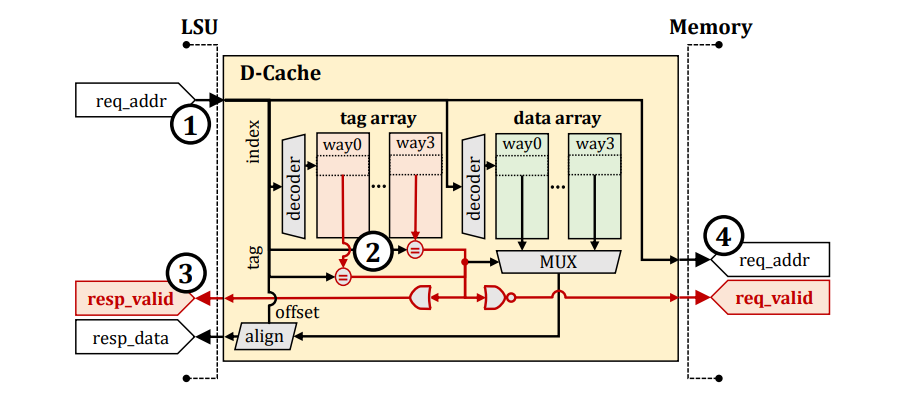
\includegraphics[width=\linewidth]{figure/proposal/specdoctor-figure5.png}
    \caption*{图5:RISC-V BOOM 处理器的 DCache 的简化逻辑。标签数组并没有和 valid 信号直接相连。}
\end{figure}

图5展示了Boom CPU的DCache中的一部分简化逻辑。DCache有两个内存组件,标签数组和数据数组。标签阵列存储内存地址的高位,而数据阵列存储内存数据。当来自 LSU 的内存读/写请求通过req\_addr信号线(即,请求的地址,1)发送给 DCache 时,DCache首先将req\_addr值与存储在标签数组(2)中的位进行比较。如果地址匹配,DCache通过使能resp\_valid信号响应LSU(1)的访存请求,2)定位存储在数据数组中的相应数据值,3)通过resp\_data信号线(3)将定位到的数据发送出去。另一方面,如果地址不匹配,DCache首先向内存(4)发送请求,然后在获取请求的数据后响应LSU。因此,标签数组是否包含匹配的地址,会通过resp\_valid信号影响DCache时间侧信道,而数据数组则不会。\par

基于这一现象,SpecDoctor设计了反向数据流分析来从被连接到上层模块的 valid 信号中识别出真正有效的时间变化组件。给定一个上层模块及其 valid 信号端口,该分析将使用从RTL源代码中解析出的电路图结构返回所有的时间变化组件。更具体地说,分析过程中SpecDoctor对每个模块进行反向分割,从而检查上层模块内部的各个子部分。以图6-(a)为例,对于具有子模块(即$m_0$,$m_1$ 和 $m_2$)的高级模块(即 M),该分析返回连接到有效端口(即$p_0$)的所有状态组件(即,$n_0$,$n_1$,$n_2$和$n_3$)。\par

\begin{figure}[!h]
    \centering
    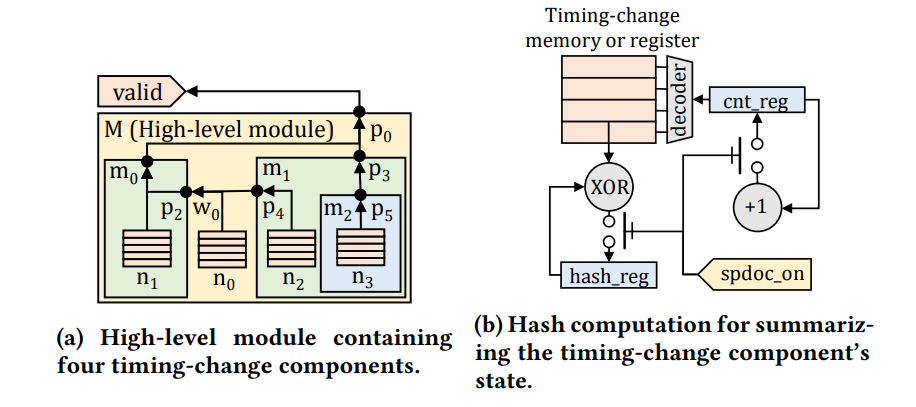
\includegraphics[width=\linewidth]{figure/proposal/specdoctor-figure6.png}
    \caption*{图6:SpecDoctor 的数据流分析和执行。}
\end{figure}

\textbf{动态地查找秘密传输指令}。在静态地识别时间变化组件后,SpecDoctor 动态地寻找可以通过时间变化组件传输秘密的指令。具体来说,SpecDoctor使用4.2中描述的算法在阶段2的测试用例的基础上随机生成瞬态指令。然后运行RTL模拟,检测指令能否根据秘密值改变时间变化组件的微观结构状态。由于时间变化组件的状态会影响指令的执行时间,因此以后可以根据时间侧信道反映这些组件的状态变化,进而推断出瞬态指令传输的秘密值。\par

为此,SpecDoctor设计了一个差分测试框架,该框架分别执行两个使用相同瞬态指令但不同秘密值(即秘密部分数据)的测试程序,然后比较RTL模拟后得到的时间变化组件的状态。注意,因为这两个测试用例在RTL模拟和其他所有内存段(即引导、代码、数据)被初始化为相同的时候,只有秘密段是不同的,所以,SpecDoctor可以确认时间变化组件的状态差异来源于两个测试用例秘密数据值的差异。换句话说,SpecDoctor可以通过检查一个给定的测试用例能否导致时间变化组件的微体系结构状态的不同来确定该测试用例能否传输秘密数据。\par

为了观察时间变化组件的微体系结构状态,SpecDoctor 会插桩每个组件并提供一个接口(例如,内存映射的spdoc\_addr)来观察它们的状态。具体来说,SpecDoctor提供了如图6-(b)所示的逻辑,当一个专用信号被使能时(即spdoc\_on)时,它打印出此时微结构状态的摘要(即hash\_reg)。在使能spdoc\_on信号后,所有时间变化组件的内存块或寄存器被分批次地通过 hash 运算保存到hash\_reg中,最终得到的hash\_reg值会被打印出来,以代表所有时间变化组件的状态。然后,我们对RTL仿真测试平台进行修改:当一个测试用例通过给定的接口(例如,存储到spdoc\_addr)修改了时间变化组件的微结构状态时,我们将使能spdoc\_on信号。\par

\begin{figure}[!h]
    \centering
    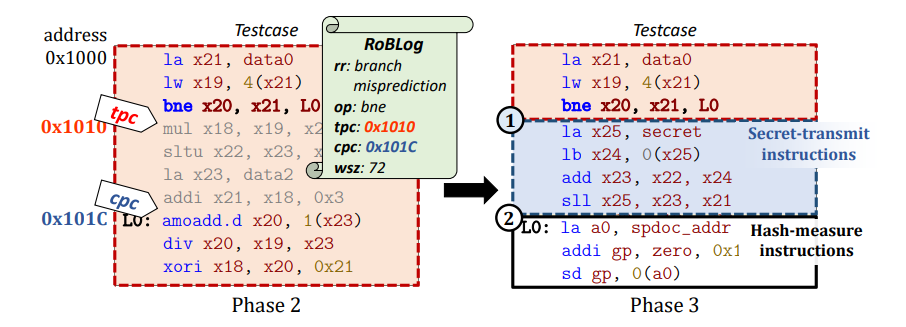
\includegraphics[width=\linewidth]{figure/proposal/specdoctor-figure7.png}
    \caption*{图7:根据SpecDoctor的RoBLog生成的第二阶段测试用例(左),以及第三阶段中生成的秘密传输指令、哈希测量指令(右)。rr:RoB回滚原因,op:触发瞬态执行的指令操作码,tpc:启动瞬态执行的指令pc,cpc:刷新瞬态执行指令后纠正得到的pc,wsz:瞬态窗口大小。}
\end{figure}

SpecDoctor 在运行随机生成的瞬态指令后,就可以通过这种方式观察组件微观结构状态的变化。例如,对于如图7左侧所示的测试用例和相应的RoBLog,SpecDoctor首先在瞬态执行指令起始pc(即RoBLog中的tpc)的位置嵌入随机生成指令,来作为该阶段的瞬态执行指令(1)。在回滚瞬态指令(即cpc,2)之后,SpecDoctor从正确的pc地址开始嵌入用于观察微架构状态的指令(即读取存储到spdoc\_addr的哈希值的访存指令),由于这部分指令是在瞬态指令回滚后立即执行的,所以SpecDoctor可以在瞬态执行后立即观察到微架构的状态。请注意,在tpc和cpc之间嵌入的瞬态执行指令并不会影响瞬态执行的触发,因为瞬态执行的触发是由前面阶段1生成的指令单独决定的。\par

\textbf{突变随机指令}。与第二阶段不同的是,SpecDoctor 在这个阶段采用了一种独特的模糊反馈技术来寻找各种秘密传输指令。具体来说,SpecDoctor维护了一个能触发状态差异的测试用例的语料库,并随机突变其中的用例以生成新的测试用例。对于测试用例的突变,SpecDoctor应用了逐条指令突变算法,该算法对给定的测试用例进行随机的指令替换、删除或附加。随机指令按照4.2中的步骤进行构造(即操作码编码和操作数嵌入)。并且 SpecDoctor只改变瞬态执行部分(即RoBLog中的tpc)的指令,这样突变就不会影响早期阶段(例如,触发瞬时执行)功能的正确执行。\par

\subsection{阶段4:接收秘密}

对于阶段3给定的秘密传递指令,阶段4找到对应的通过时间侧信道接收秘密的秘密接受指令。具体来说,我们设计了另一个差分测试,它使用不同的秘密执行两次测试用例,并比较所使用的CPU周期。当运行这两个测试用例时,除了秘密部分以外的其他所有输入部分(即,指令和内存部分)都被初始化为相同的值。SpecDoctor通过这种方式确保两次指令执行之间的时间差异仅由秘密数据的差异决定。\par

\textbf{寻找秘密接收指令。}为了找到秘密接收指令,SpecDoctor 在代码部分嵌入随机生成指令,并且测量执行这些指令之前和之后的时钟计数,进而得到这部分代码的执行时间。测试用例模板的秘密接收指令是在阶段1到阶段3生成的所有指令执行生效的基础上的执行的,所以当秘密接收指令执行时,时间变化组件的微体系结构状态已经被秘密传输指令所改变了。此外,秘密接收指令只能在攻击者的特权下执行,因为秘密接收只会在攻击者一方的上下文执行。然后,SpecDoctor比较测量得到的RTL模拟的时钟周期计数(即指令执行时间)的差异,如果差异存在,则说明确定接收到了秘密。\par

最终,1)触发瞬时执行的汇编指令,2)瞬时访问和秘密传输的汇编指令,以及3)秘密接收的汇编指令组成的汇编文件会被完整保存起来,作为瞬时执行攻击的PoC。

% \sectionnonum{摘要}

% \section{节标题}


% 参考~\cite{zjuthesisrules, zjuthesis}

% \begingroup
%     \linespreadsingle{}
%     \printbibliography[title={外文翻译参考文献}]
% \endgroup
